\subsection{Thực nghiệm và kết quả định vị của mô hình YOLO11s}
\label{subsec:kq_yolo}

Khâu định vị đối tượng (Tầng 1) giữ vai trò then chốt trong việc xác lập chặn trên hiệu năng toàn trình (End-to-End Recall) của toàn hệ thống. Mọi thực nghiệm của detector được tiến hành trên tập kiểm thử độc lập (Blind Test) gồm \textbf{550 ảnh hiện trường} (tương ứng 1.845 nhãn ground-truth tổng thể, trong đó có \textbf{1.821 nhãn ground-truth} thuộc 5 nhóm biển báo chính quy chuẩn QCVN 41:2019 và 24 nhãn camera ngoại lai).

\subsubsection{Năng lực Zero-shot và hiệu quả chuyển giao miền dữ liệu (Domain Adaptation)}
\label{subsubsec:yolo_zeroshot_finetune}

Để kiểm chứng giá trị của chiến lược học chuyển giao đa tầng (COCO $\rightarrow$ CCTSDB $\rightarrow$ Việt Nam), mô hình tiền huấn luyện trên dữ liệu biển báo Trung Quốc \texttt{cctsdb\_s} được kiểm thử trực tiếp trên tập Test Việt Nam khi \textbf{chưa từng được học bất kỳ ảnh giao thông Việt Nam nào (Zero-shot evaluation)}, sau đó đối chứng trực tiếp với mô hình đã hoàn tất tinh chỉnh miền \texttt{vn\_s}:

\begin{table}[H]
\centering
\small
\caption{Đối chứng hiệu năng Zero-shot (\texttt{cctsdb\_s}) và Finetune (\texttt{vn\_s}) trên tập Test Việt Nam.}
\label{tab:yolo_zeroshot_vs_finetune}
\begin{tabularx}{\textwidth}{|p{3.2cm}|>{\centering\arraybackslash}p{2.5cm}|>{\centering\arraybackslash}X|>{\centering\arraybackslash}X|>{\centering\arraybackslash}X|>{\centering\arraybackslash}X|}
\hline
\textbf{Mô hình} & \textbf{Cấu hình đo kiểm} & \textbf{Precision} & \textbf{Recall} & \textbf{mAP50} & \textbf{mAP50-95} \\
\hline
\multirow{2}{*}{\texttt{cctsdb\_s} (Zero-shot)} & Runtime ($\text{conf} = 0.25$) & 91.86\% & 71.54\% & 70.49\% & 52.70\% \\
\cline{2-6}
& Benchmark ($\text{conf} = 0.001$) & 88.85\% & 74.28\% & 81.33\% & 58.52\% \\
\hline
\multirow{2}{*}{\textbf{\texttt{vn\_s} (Finetune chuẩn)}} & \textbf{Runtime ($\text{conf} = 0.25$)} & \textbf{92.24\%} & \textbf{82.93\%} & \textbf{83.63\%} & \textbf{60.11\%} \\
\cline{2-6}
& \textbf{Benchmark ($\text{conf} = 0.001$)} & \textbf{92.19\%} & \textbf{82.87\%} & \textbf{90.32\%} & \textbf{63.53\%} \\
\hline
\textbf{Mức cải thiện ròng} & Runtime ($\text{conf} = 0.25$) & \textbf{+0.38\%} & \textbf{+11.39\%} & \textbf{+13.14\%} & \textbf{+7.41\%} \\
\hline
\end{tabularx}
\end{table}

\textbf{Làm rõ sự khác biệt giữa hai con số mAP50 (83.63\% so với 90.32\%):}
\begin{itemize}
    \item \textbf{Con số 83.63\% (Runtime):} Thu được từ kịch bản đánh giá thực tế của hệ thống với ngưỡng tự tin vận hành $\text{conf} = 0.25$ và $\text{IoU} = 0.6$. Ngưỡng này phản ánh chính xác chất lượng hộp bao thực tế chuyển tiếp sang Tầng 2.
    \item \textbf{Con số 90.32\% (Benchmark):} Xuất phát từ giao thức chuẩn hóa của thư viện Ultralytics (tương đương chuẩn đánh giá MS COCO / PASCAL VOC), quét ngưỡng tự tin cực thấp $\text{conf} = 0.001$ để tích phân toàn bộ diện tích dưới đường cong Precision-Recall (AUC).
\end{itemize}
Việc tinh chỉnh trên dữ liệu Việt Nam giúp Recall thực tế tăng vọt từ $71.54\%$ lên $82.93\%$ (trên tổng số nhãn bao gồm cả Camera) và đạt \textbf{85.61\% (1.559 / 1.821)} trên 5 nhóm biển báo chính quy chuẩn, với mAP50 thực tế tăng $+13.14$ điểm phần trăm.

\subsubsection{Phân tích độ phủ phát hiện theo kích thước và nhóm biển báo}
\label{subsubsec:yolo_breakdown}

Tại ngưỡng vận hành $\text{conf} = 0.25$, mô hình \texttt{vn\_s} phát hiện thành công \textbf{1.559 / 1.821 biển báo chính} (đạt Recall \textbf{85.61\%}) và tạo ra \textbf{216 báo động giả (FP)}.

\begin{figure}[H]
\centering
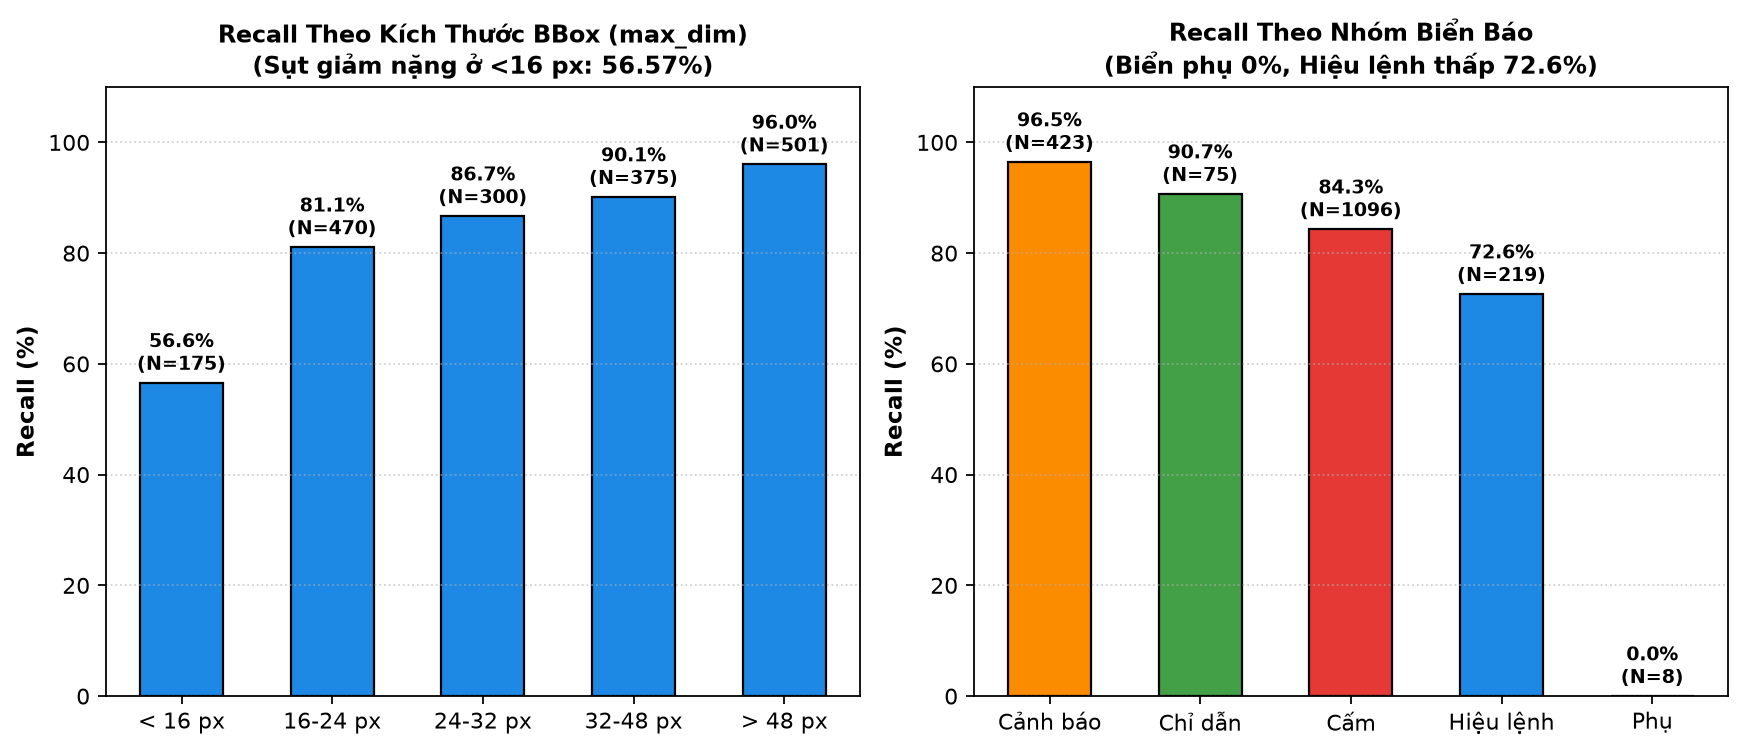
\includegraphics[width=0.92\textwidth]{graphics/sec4/f2_11_diag_recall_breakdown.png}
\caption{Phân tích độ phủ phát hiện (Recall \%) của detector \texttt{vn\_s} phân theo dải kích thước hình học (trái) và phân theo 5 nhóm biển báo quy chuẩn (phải).}
\label{fig:diag_recall_breakdown}
\end{figure}

\textbf{Đọc Hình~\ref{fig:diag_recall_breakdown}:}
Biểu đồ phân đoạn bên trái cho thấy sự phụ thuộc chặt chẽ giữa kích thước biển báo và độ nhạy phát hiện: các biển lớn ($> 48\text{ px}$) đạt tỷ lệ bắt trúng áp đảo \textbf{95.98\%} (478/498) và biển trung bình ($32-48\text{ px}$) đạt \textbf{90.21\%} (341/378); tuy nhiên khi kích thước giảm xuống dải siêu nhỏ ($< 16\text{ px}$), tỷ lệ phát hiện tụt dốc còn \textbf{56.57\%} (99/175). Biểu đồ bên phải thể hiện độ phủ vượt trội trên nhóm biển Cảnh báo (\textbf{96.45\%}) và Chỉ dẫn (\textbf{90.67\%}), trong khi nhóm Cấm đạt \textbf{84.31\%}, nhóm Hiệu lệnh đạt \textbf{72.60\%} và nhóm Biển phụ đạt \textbf{0.0\%} (0/8 mẫu, do kích thước quá nhỏ và dạng hình chữ nhật dẹt dễ lẫn vào nền).

\subsubsection{Kiểm chứng thực nghiệm với hai biến thể mở rộng (\texttt{vn\_s\_1024} và \texttt{vn\_s\_tt100k})}
\label{subsubsec:yolo_variants}

Để kiểm định hai giả định kỹ thuật: (1) nâng độ phân giải đầu vào lên $1024 \times 1024$ giúp bắt biển nhỏ tốt hơn, và (2) sử dụng tập dữ liệu ảnh vuông TT100K làm tiền huấn luyện mang lại biểu diễn nhạy bén hơn, hai mô hình thử nghiệm được huấn luyện độc lập với nguyên tắc đổi duy nhất một biến số so với baseline \texttt{vn\_s}.

\begin{figure}[H]
\centering
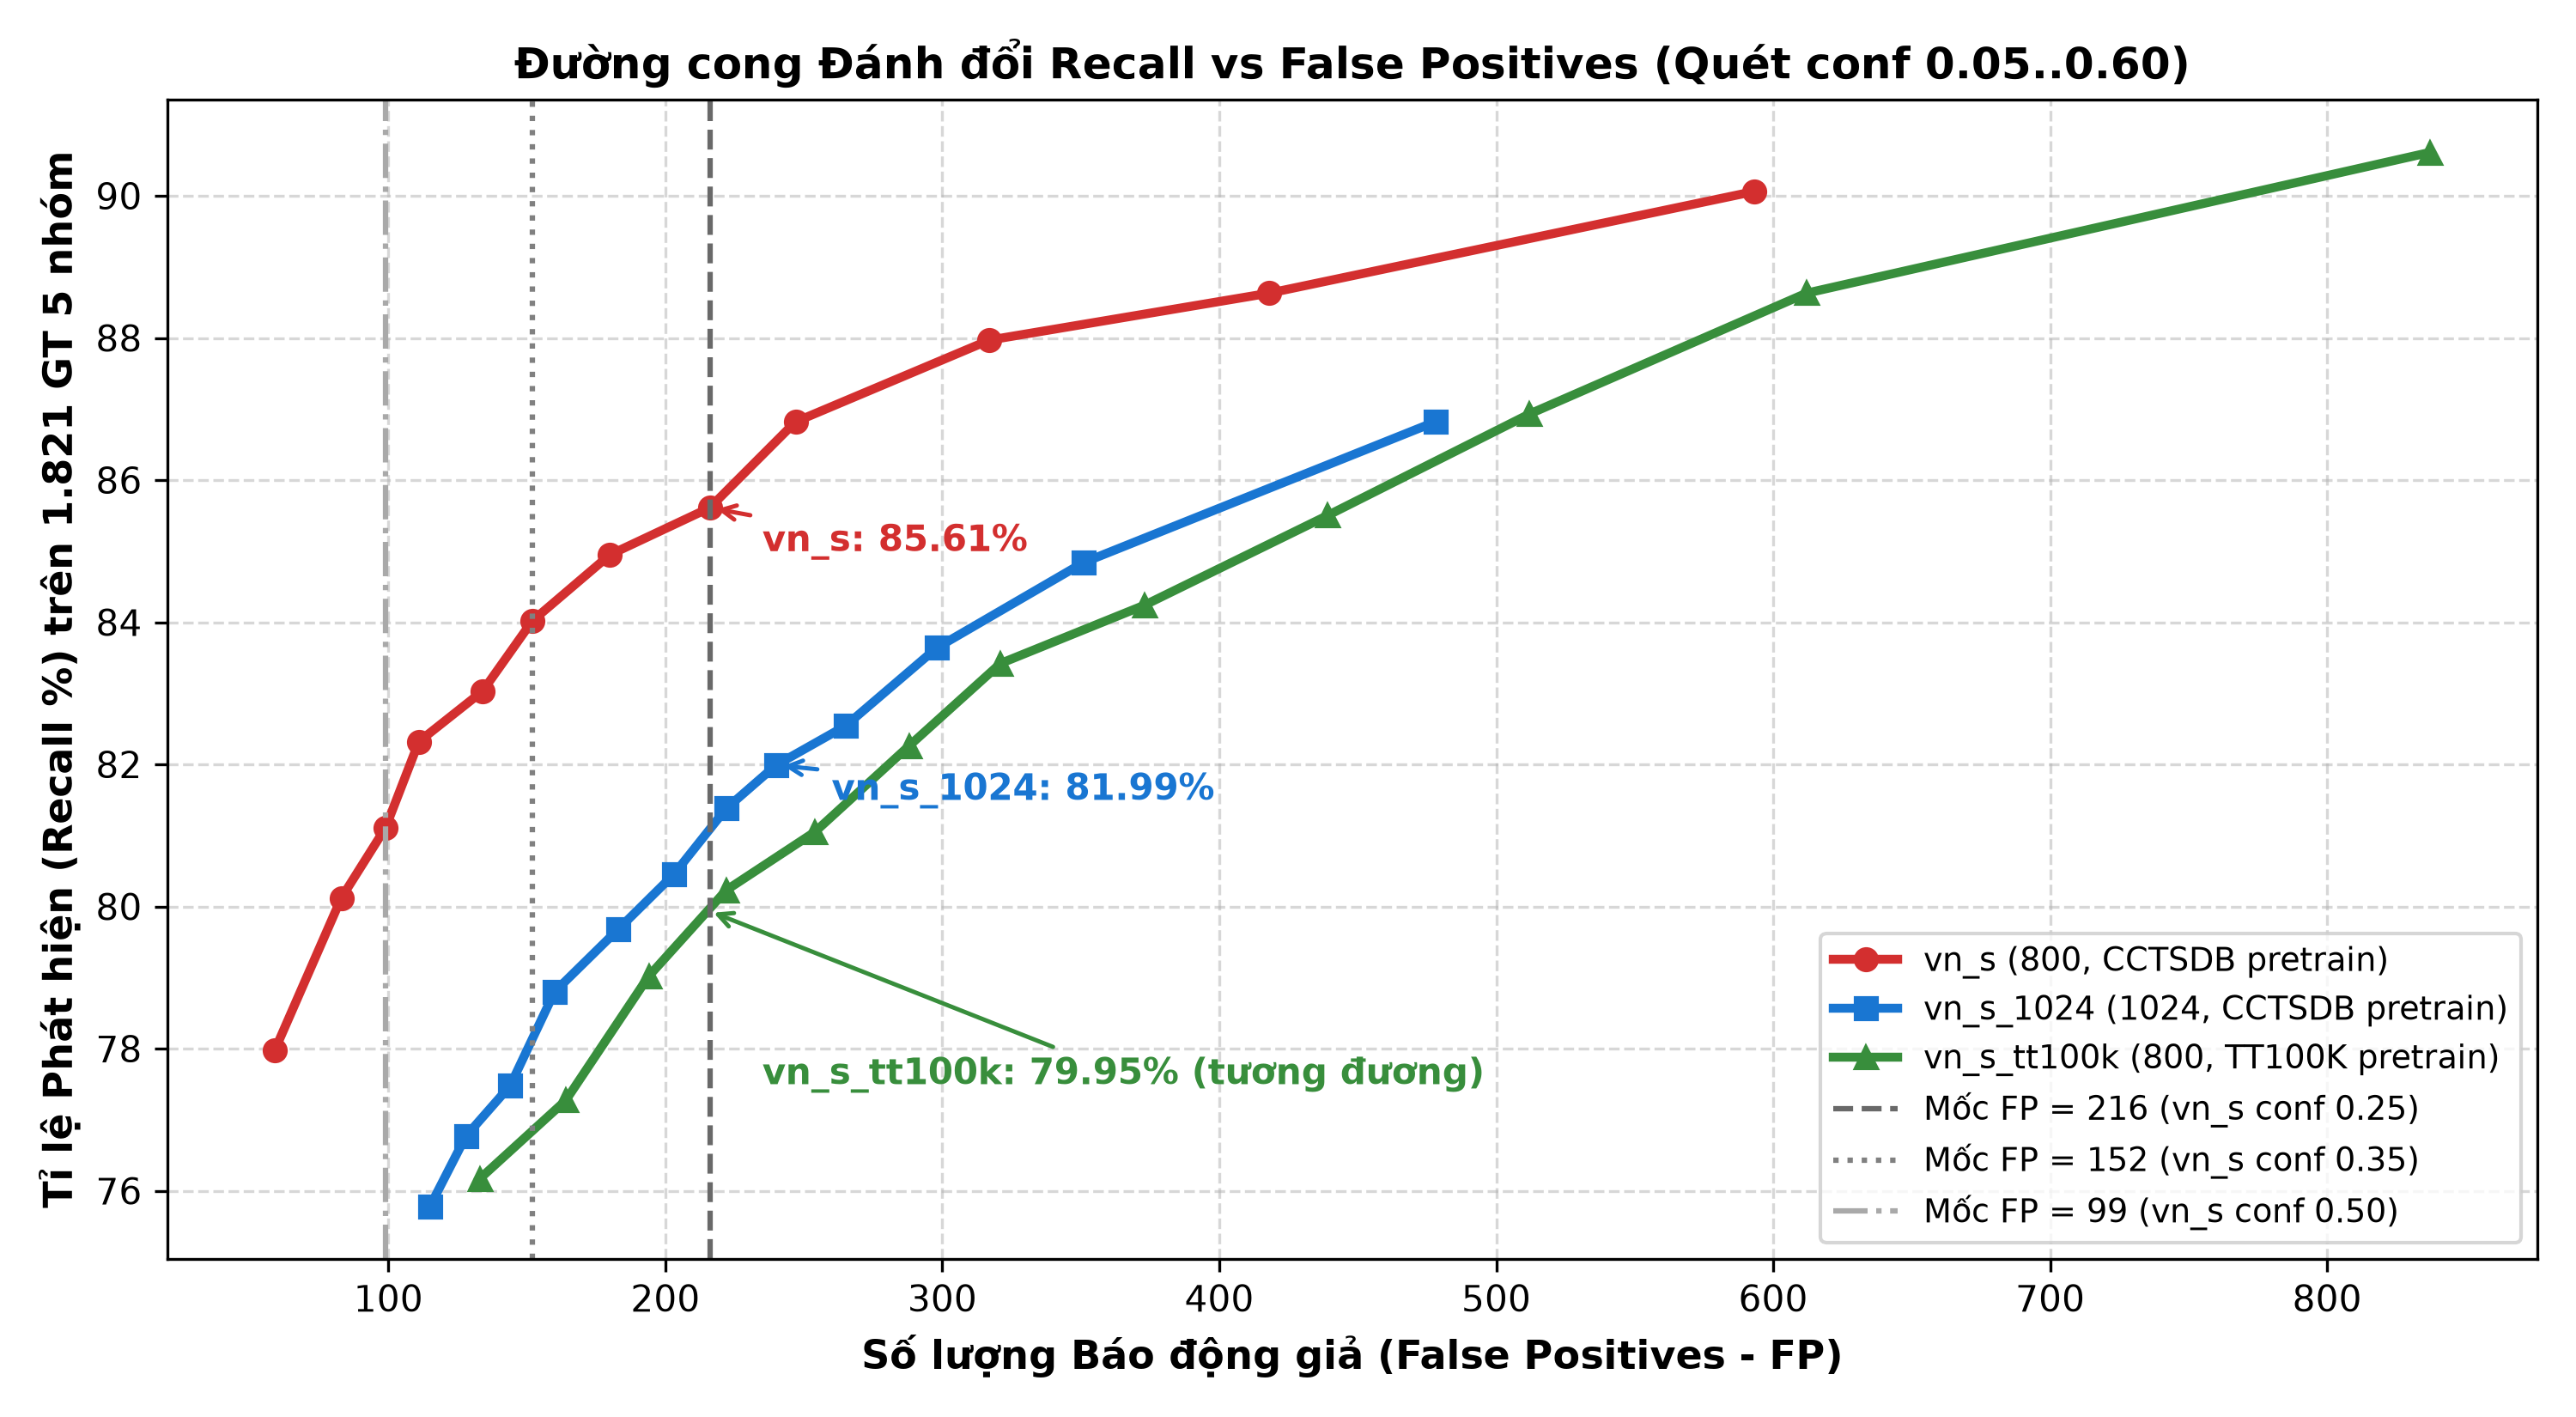
\includegraphics[width=0.88\textwidth]{graphics/sec4/f2_14_recall_vs_fp_curves.png}
\caption{Đường cong đánh đổi giữa Recall (\%) và số lượng False Positives (FP) trên tập Test Việt Nam khi quét ngưỡng tự tin từ $0.05$ đến $0.60$.}
\label{fig:recall_vs_fp_curves}
\end{figure}

\textbf{Đọc Hình~\ref{fig:recall_vs_fp_curves}:}
Trên toàn dải quét số lượng báo động giả từ 50 đến 600 FP, đường cong của baseline \texttt{vn\_s} (đường màu cam) luôn nằm cao hơn hẳn hai biến thể \texttt{vn\_s\_1024} (màu xanh dương) và \texttt{vn\_s\_tt100k} (màu xanh lá). Để đảm bảo tính khách quan khoa học, bảng đối chứng dưới đây thực hiện so sánh công bằng tại các mốc FP cố định:

\begin{table}[H]
\centering
\small
\caption{So sánh đối chuẩn Recall công bằng tại cùng mức báo động giả cố định (False Positives).}
\label{tab:yolo_fair_fp_comparison}
\begin{tabularx}{\textwidth}{|p{3.8cm}|>{\centering\arraybackslash}p{2.0cm}|>{\centering\arraybackslash}p{2.0cm}|>{\centering\arraybackslash}p{2.6cm}|>{\centering\arraybackslash}X|}
\hline
\textbf{Mốc đối chuẩn kiểm soát} & \textbf{Số FP chuẩn} & \textbf{Recall \texttt{vn\_s}} & \textbf{Recall \texttt{vn\_s\_1024}} & \textbf{Recall \texttt{vn\_s\_tt100k}} \\
\hline
Tại mốc $\text{conf} = 0.25$ của \texttt{vn\_s} & \textbf{216 FP} & \textbf{85.61\%} & 81.04\% ($-4.57\%$) & 79.95\% ($-5.66\%$) \\
\hline
Tại mốc $\text{conf} = 0.35$ của \texttt{vn\_s} & \textbf{152 FP} & \textbf{84.02\%} & 78.43\% ($-5.59\%$) & 77.08\% ($-6.94\%$) \\
\hline
Tại mốc $\text{conf} = 0.50$ của \texttt{vn\_s} & \textbf{99 FP} & \textbf{81.11\%} & 75.12\% ($-5.99\%$) & 76.17\% ($-4.94\%$) \\
\hline
\end{tabularx}
\end{table}

\textbf{Nhận xét và kết luận lựa chọn (Đánh giá trung tính, 1 lần chạy, 1 seed):}
\begin{itemize}
    \item Thực nghiệm chứng minh tại mọi mức FP kiểm soát, mô hình \texttt{vn\_s} đều đạt Recall cao hơn biến thể \texttt{vn\_s\_1024} từ $4.57\%$ đến $5.99\%$ và cao hơn \texttt{vn\_s\_tt100k} từ $4.94\%$ đến $6.94\%$. Đặc biệt tại phân đoạn biển siêu nhỏ ($< 16\text{ px}$), \texttt{vn\_s} đạt $56.57\%$ trong khi \texttt{vn\_s\_1024} chỉ đạt $43.43\%$ và \texttt{vn\_s\_tt100k} chỉ đạt $40.00\%$.
    \item \textit{Nguyên nhân suy giảm hiệu năng của mô hình 1024 và TT100K: giả định, chưa kiểm chứng.} Có thể do sự bất tương xứng tỉ lệ khung hình (domain scale shift) giữa tập dữ liệu pretrain và tập dữ liệu mục tiêu khiến lưới anchor/receptive field học sai phân bố kích thước.
    \item \textbf{Quyết định:} Nhóm quyết định giữ nguyên mô hình \textbf{\texttt{vn\_s} (imgsz 800, pretrain CCTSDB)} làm detector chính thức cho toàn bộ pipeline vì đạt độ phủ cao nhất, chi phí tính toán thấp hơn và tiết kiệm khoảng $45\%$ thời gian suy luận so với cấu hình 1024.
\end{itemize}

\subsubsection{Phân tích định tính các ca phát hiện mẫu (GT, TP, FN, FP)}
\label{subsubsec:yolo_qualitative}

\begin{figure}[H]
\centering
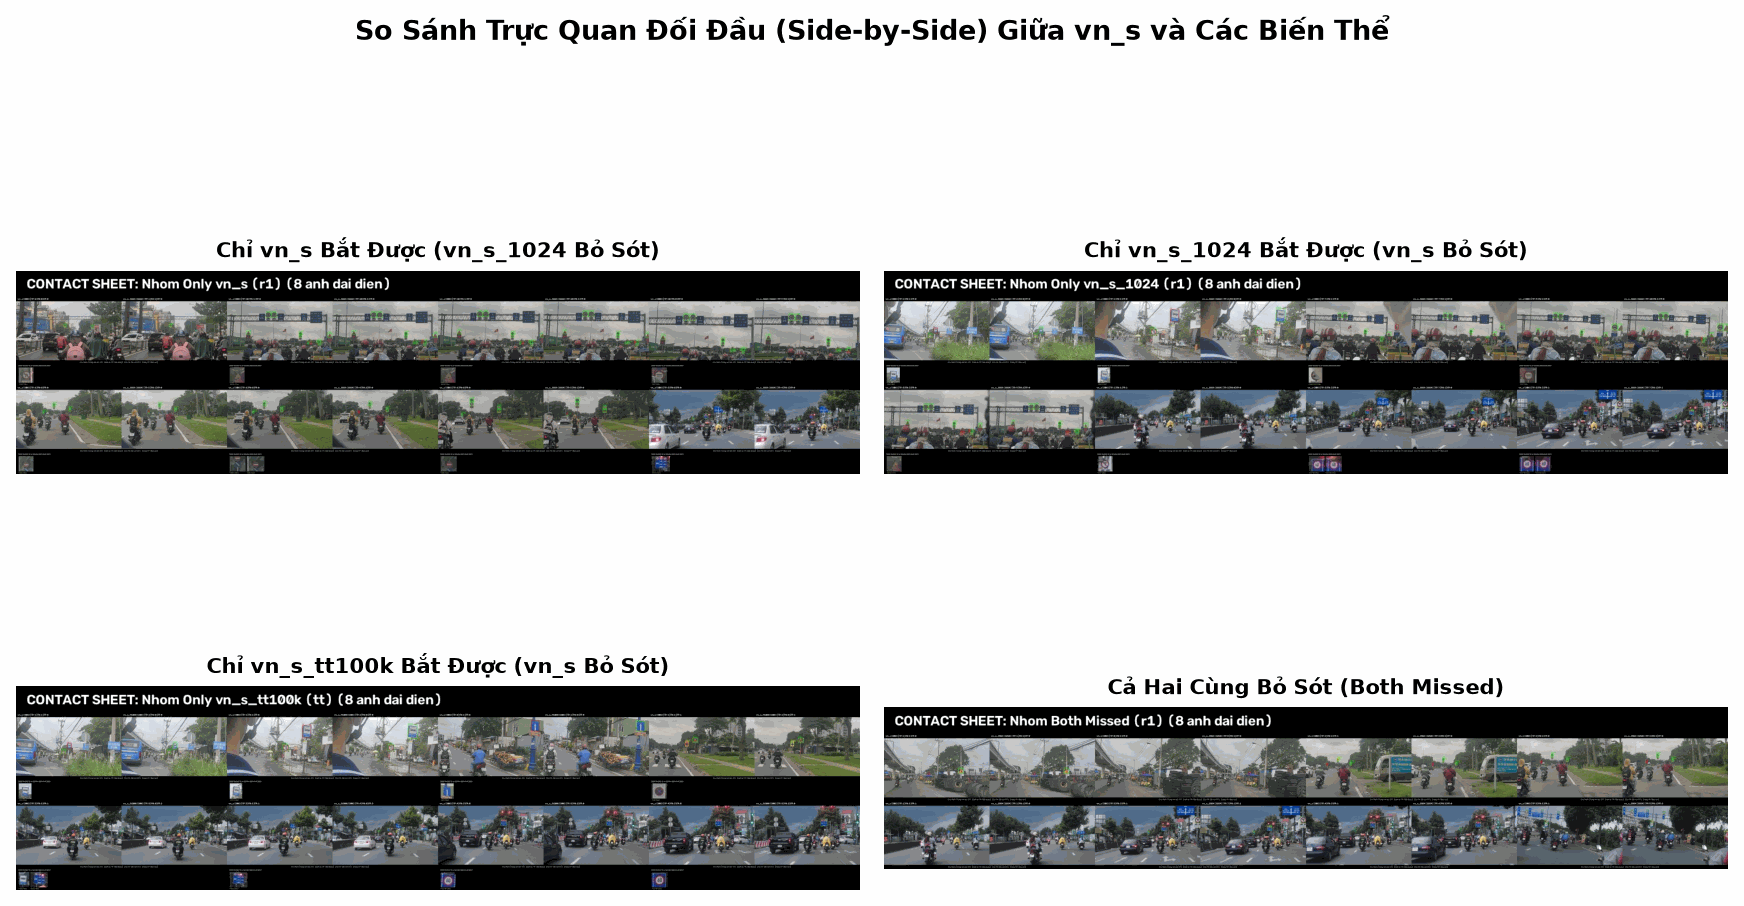
\includegraphics[width=0.92\textwidth]{graphics/sec4/f2_16_side_by_side_and_tracks.png}
\caption{Minh họa thực tế các ca phát hiện trên tập Test: so sánh đối đầu phát hiện giữa các mô hình (trên) và diễn biến bắt vết biển vật lý theo chuỗi khung hình camera hành trình (dưới).}
\label{fig:side_by_side_tracks}
\end{figure}

\textbf{Đọc Hình~\ref{fig:side_by_side_tracks}:}
Hàng trên minh họa các tình huống bắt độc lập: \texttt{vn\_s} phát hiện thành công các biển báo xa bị nhòe mờ mà các mô hình đối chứng bỏ sót. Hàng dưới thể hiện tính bám vết liên tục theo thời gian: khi xe tiến lại gần từ khoảng cách xa, kích thước biển báo tăng dần từ dưới $15\text{ px}$ lên trên $35\text{ px}$, điểm tự tin của detector tăng đều đặn từ $0.30$ lên trên $0.85$.

\begin{figure}[H]
\centering
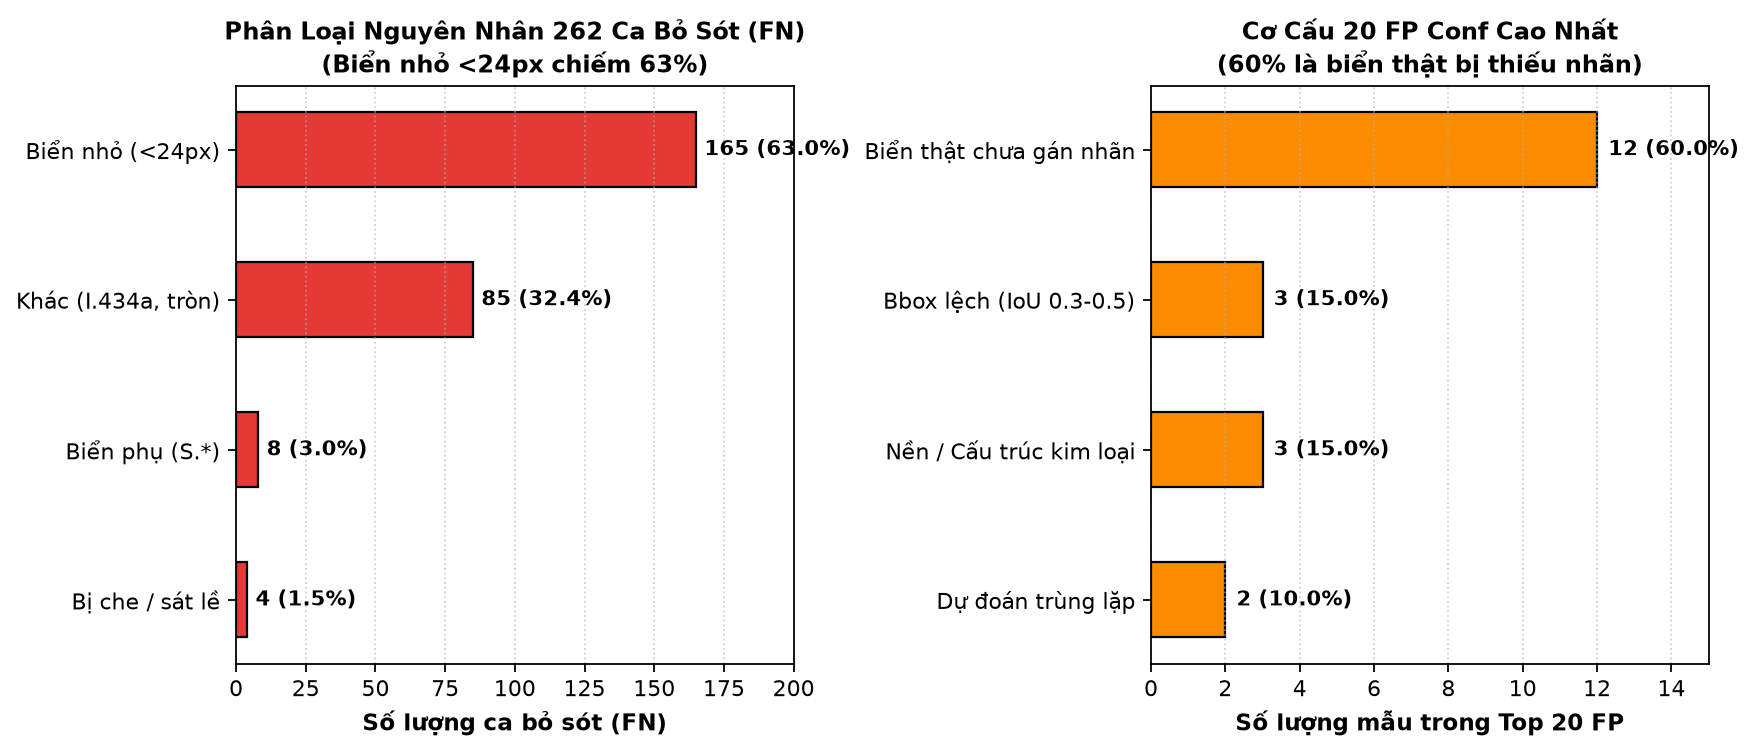
\includegraphics[width=0.92\textwidth]{graphics/sec4/f2_12_fn_taxonomy_and_fp20.png}
\caption{Chẩn đoán trực quan lỗi định vị của \texttt{vn\_s}: phân loại các hình thái bỏ sót (FN, trái) và kiểm toán trực quan 20 trường hợp báo động giả (FP, phải).}
\label{fig:fn_taxonomy_fp20}
\end{figure}

\textbf{Đọc Hình~\ref{fig:fn_taxonomy_fp20}:}
Phân loại lỗi bỏ sót (trái) chỉ ra $63.0\%$ số ca FN tập trung ở kích thước siêu nhỏ $< 24\text{ px}$, bị cành cây rậm che khuất hoặc chụp ở góc nghiêng lớn. Kiểm toán trực quan top 20 False Positive (phải) hé lộ một hiện tượng quan trọng: \textbf{12/20 trường hợp (chiếm 60\% mẫu khảo sát)} thực chất là biển báo giao thông có thật ngoài hiện trường nhưng bị thiếu nhãn trong tập ground-truth ban đầu.

% =========================================================================================
\subsection{Thực nghiệm và kết quả phân loại đặc trưng HSV + HOG + SVM}
\label{subsec:kq_hsv_svm}

Tầng phân loại truyền thống tiếp nhận các vùng ảnh con ROI được cắt từ hộp bao của detector, trích xuất vector đặc trưng đa tầng $S0 \rightarrow S1 \rightarrow S2 \rightarrow S3$ và phân loại thành các nhóm biển báo quy chuẩn.

\subsubsection{Phân bố không gian màu sắc HSV theo nhóm biển báo}
\label{subsubsec:hsv_distributions}

\begin{figure}[H]
\centering
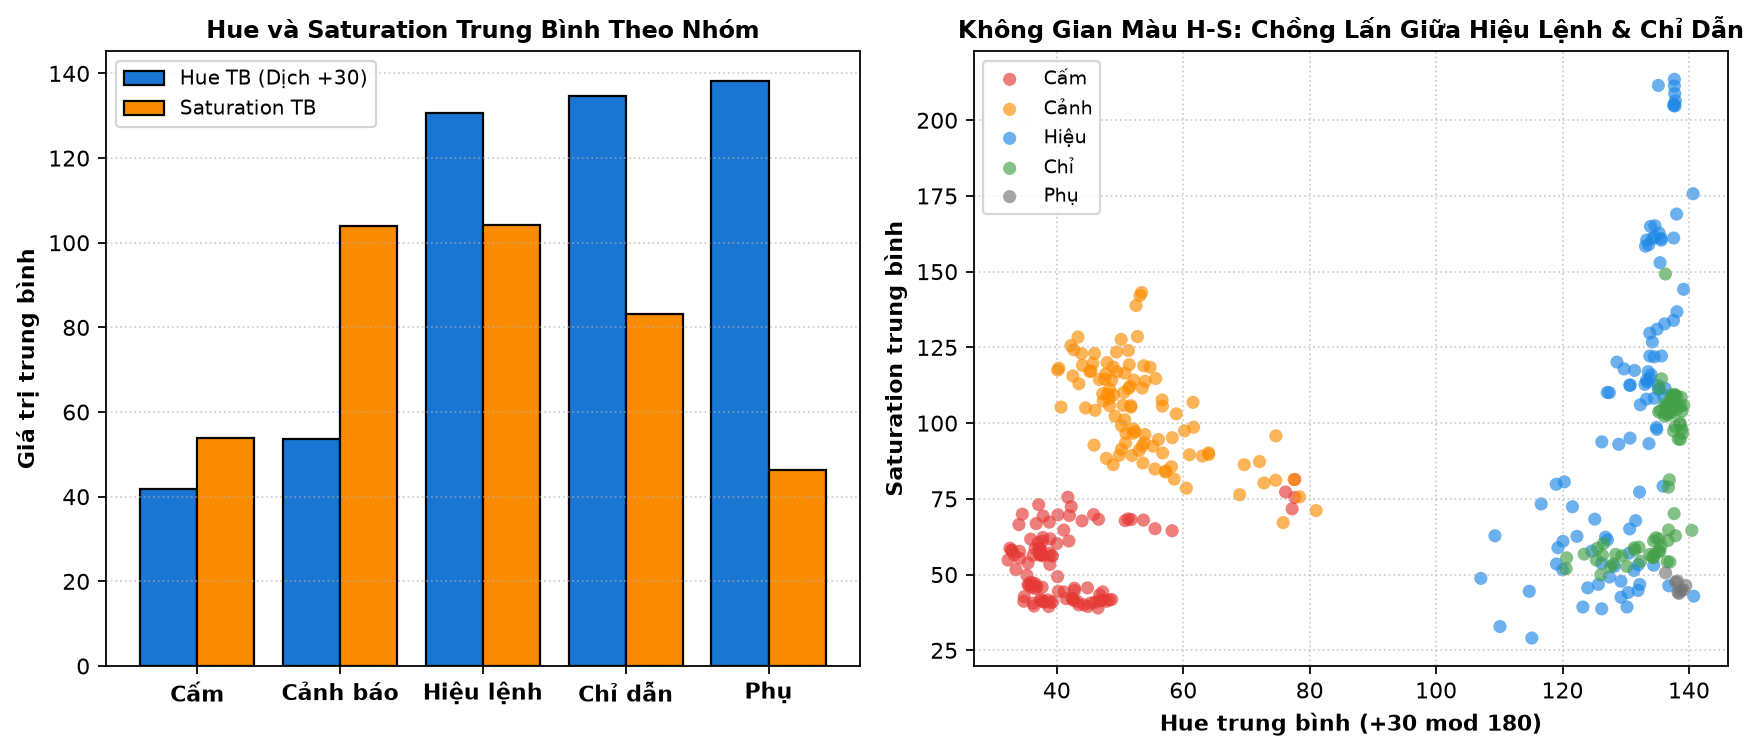
\includegraphics[width=0.92\textwidth]{graphics/sec4/f1_09_hsv_hist_and_hs_scatter.png}
\caption{Phân tích phân bố không gian màu HSV trên tập dữ liệu Việt Nam: biểu đồ tần suất kênh Hue (trên) và biểu đồ phân tán Hue-Saturation theo nhóm biển báo (dưới).}
\label{fig:hsv_hist_scatter}
\end{figure}

\textbf{Đọc Hình~\ref{fig:hsv_hist_scatter}:}
Hàng trên làm rõ cơ sở vật lý của kỹ thuật dịch vòng $+30^\circ$: kênh Hue dịch chuyển giúp gom dải đỏ thành một cụm đơn đỉnh duy nhất tại khoảng $30^\circ - 50^\circ$, tách biệt hoàn toàn khỏi đỉnh xanh lam của nhóm Hiệu lệnh và Chỉ dẫn tại khoảng $120^\circ - 150^\circ$. Tuy nhiên, biểu đồ phân tán (hàng dưới) cũng làm sáng tỏ điểm nghẽn nghiêm trọng: nhóm Hiệu lệnh (xanh tròn) và nhóm Chỉ dẫn (xanh chữ nhật) có phân bố màu sắc gần như trùng khít hoàn toàn trong không gian HS, giải thích nguyên nhân các bộ phân loại chỉ dùng màu sắc toàn cục ($S0$) luôn thất bại trong việc phân biệt hai nhóm này.

\subsubsection{Thẩm định chéo GroupKFold trên chuỗi đặc trưng \texorpdfstring{$S0 \rightarrow S3$}{S0 -> S3}}
\label{subsubsec:groupkfold_s0_s3}

Để ngăn chặn hiện tượng rò rỉ dữ liệu giữa các frame kề nhau, quá trình kiểm chứng chéo 5-fold được nhóm theo 20 cụm video độc lập (\texttt{GroupKFold}). Bảng~\ref{tab:groupkfold_all_results} tổng hợp kết quả chi tiết của 5 thuật toán học máy qua các nấc đặc trưng:

\begin{table}[H]
\centering
\small
\caption{Kết quả kiểm chứng chéo GroupKFold (mean $\pm$ std) và đánh giá trên tập Test Mức A.}
\label{tab:groupkfold_all_results}
\begin{tabularx}{\textwidth}{|p{3.2cm}|>{\centering\arraybackslash}p{1.4cm}|p{2.6cm}|>{\centering\arraybackslash}p{2.8cm}|>{\centering\arraybackslash}p{1.8cm}|>{\centering\arraybackslash}X|}
\hline
\textbf{Nấc đặc trưng} & \textbf{Số chiều} & \textbf{Mô hình} & \textbf{GroupKFold Macro-F1} & \textbf{Test Acc (Mức A)} & \textbf{Test Macro-F1 (Mức A)} \\
\hline
\multirow{5}{*}{$S0$ (H36+S8)} & \multirow{5}{*}{44} & SVM (RBF) & $0.6521 \pm 0.0570$ & 94.78\% & 0.8315 \\
& & kNN ($k=11$) & $0.6309 \pm 0.0494$ & 95.39\% & 0.8328 \\
& & Random Forest & $0.6820 \pm 0.0656$ & 98.46\% & 0.8789 \\
& & XGBoost & $0.6828 \pm 0.0499$ & 97.53\% & 0.8627 \\
& & LightGBM & $0.6782 \pm 0.0415$ & 98.02\% & 0.8798 \\
\hline
\multirow{5}{*}{$S1$ ($+$w/h)} & \multirow{5}{*}{45} & SVM (RBF) & $0.6608 \pm 0.0644$ & 95.44\% & 0.8665 \\
& & kNN ($k=11$) & $0.6537 \pm 0.0557$ & 96.32\% & 0.8657 \\
& & Random Forest & $0.6898 \pm 0.0666$ & 98.30\% & 0.8669 \\
& & XGBoost & $0.6948 \pm 0.0607$ & 98.02\% & 0.8872 \\
& & LightGBM & $0.7022 \pm 0.0497$ & 98.19\% & 0.9199 \\
\hline
\multirow{5}{*}{$S2$ ($+$grid $2\times2$)} & \multirow{5}{*}{133} & SVM (RBF) & $0.7130 \pm 0.1048$ & 97.47\% & 0.9279 \\
& & kNN ($k=11$) & $0.6727 \pm 0.0727$ & 95.55\% & 0.8468 \\
& & Random Forest & $0.7304 \pm 0.0814$ & 99.29\% & 0.9556 \\
& & XGBoost & $0.7566 \pm 0.0826$ & 98.68\% & 0.9476 \\
& & LightGBM & $0.7628 \pm 0.0792$ & 98.90\% & 0.9507 \\
\hline
\multirow{5}{*}{\textbf{$S3$ ($+$HOG)}} & \multirow{5}{*}{\textbf{457}} & \textbf{SVM (RBF, Best)} & $\mathbf{0.8983 \pm 0.0746}$ & \textbf{98.57\%} & \textbf{0.9640} \\
& & kNN ($k=11$) & $0.8455 \pm 0.1113$ & 98.24\% & 0.9687 \\
& & Random Forest & $0.8753 \pm 0.0981$ & 98.68\% & 0.9624 \\
& & XGBoost & $0.8838 \pm 0.0851$ & 98.68\% & 0.9421 \\
& & LightGBM & $0.8885 \pm 0.0882$ & 98.74\% & 0.9517 \\
\hline
\end{tabularx}
\end{table}

\begin{figure}[H]
\centering
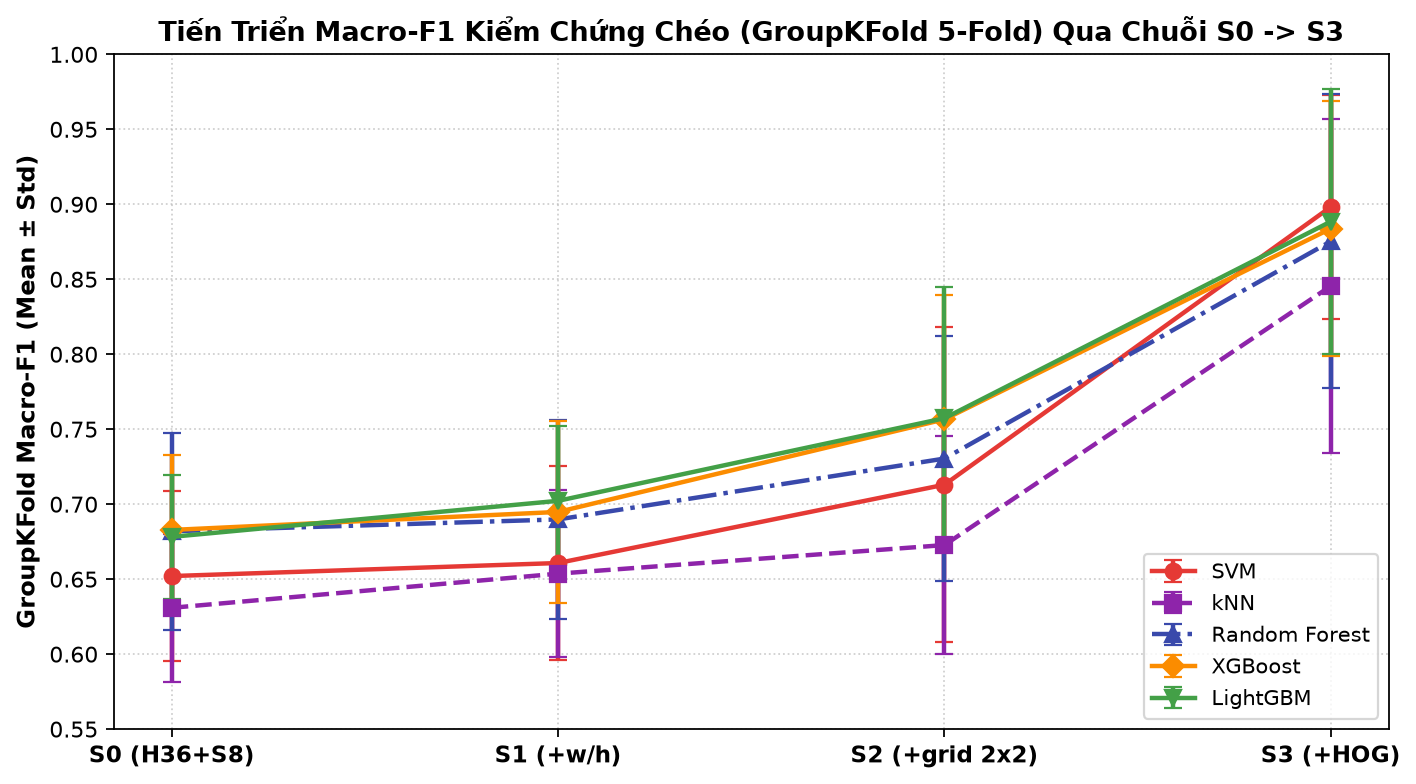
\includegraphics[width=0.90\textwidth]{graphics/sec4/f1_16_chain_progression_all_models.png}
\caption{Tiến triển chỉ số GroupKFold Macro-F1 (kèm thanh sai số $\pm 1\sigma$) qua các nấc trích xuất đặc trưng cho cả 5 mô hình phân loại.}
\label{fig:chain_progression}
\end{figure}

\textbf{Đọc Hình~\ref{fig:chain_progression}:}
Đồ thị thể hiện bước nhảy vọt hiệu năng khi chuyển từ $S2$ sang $S3$: việc tích hợp đặc trưng HOG bổ sung 324 chiều cấu trúc hình thái học giúp GroupKFold Macro-F1 của SVM tăng mạnh từ $0.7130$ lên \textbf{0.8983} (tăng $+0.1853$, tương ứng cải thiện tuyệt đối \textbf{+24.62\%} so với mốc xuất phát $S0$). Các mô hình Boosting như LightGBM ($0.8885$) và XGBoost ($0.8838$) bám sát phía sau; kiểm định bắt cặp từng fold cho thấy chênh lệch giữa SVM và Boosting nằm trong khoảng rung sai số ($\mu_{\text{diff}} < \sigma_{\text{diff}}$), tức chưa phân biệt được về mặt ý nghĩa thống kê. Về tốc độ suy luận thuần túy trên CPU (trên vector 457 chiều), XGBoost đạt $0.018\text{ ms/crop}$ và LightGBM đạt $0.021\text{ ms/crop}$, nhanh hơn xấp xỉ 30 lần so với SVM ($0.612\text{ ms/crop}$).

\subsubsection{Đánh giá trên tập kiểm thử cố định qua 3 cấp độ (Mức A, Mức A', Mức B)}
\label{subsubsec:levels_a_b}

Để đánh giá tính chịu lỗi của bộ phân loại khi hoạt động trong điều kiện hộp bao bị lệch tâm hoặc lẫn nền do detector tạo ra, hệ thống thiết lập 3 cấp độ đối chuẩn công bằng:

\begin{table}[H]
\centering
\small
\setlength{\tabcolsep}{3.5pt}
\caption{Đánh giá công bằng qua 3 cấp độ: Mức A (1.821 GT sạch), Mức A' (1.559 GT tương ứng với phát hiện), và Mức B (1.559 crop thực tế do YOLO sinh ra).}
\label{tab:levels_a_aprime_b}
\begin{tabularx}{\textwidth}{|p{2.3cm}|p{2.3cm}|>{\centering\arraybackslash}X|>{\centering\arraybackslash}X|>{\centering\arraybackslash}X|>{\centering\arraybackslash}X|>{\centering\arraybackslash}X|>{\centering\arraybackslash}X|}
\hline
\textbf{Nấc đặc trưng} & \textbf{Mô hình tốt nhất} & \textbf{Acc (A)} & \textbf{F1 (A)} & \textbf{Acc (A')} & \textbf{F1 (A')} & \textbf{Acc (B)} & \textbf{F1 (B)} \\
\hline
$S0$ (H36+S8) & Random Forest & 98.46\% & 0.8789 & 99.10\% & 0.7760 & 98.20\% & 0.7732 \\
\hline
$S1$ ($+$w/h) & Random Forest & 98.30\% & 0.8669 & 99.10\% & 0.7771 & 98.14\% & 0.7746 \\
\hline
$S2$ ($+$grid $2\times2$) & Random Forest & 99.29\% & 0.9556 & 99.74\% & 0.7954 & 99.55\% & 0.7948 \\
\hline
\textbf{$S3$ ($+$HOG)} & \textbf{SVM (RBF)} & \textbf{98.57\%} & \textbf{0.9640} & \textbf{99.29\%} & \textbf{0.9738} & \textbf{99.17\%} & \textbf{0.9687} \\
\hline
\end{tabularx}
\end{table}

\textbf{Hiệu năng toàn trình (End-to-End Recall):}
Khi chuyển từ hộp bao lý tưởng ($A'$) sang ảnh crop thực tế từ YOLO ($B$), Macro-F1 của $S3$ SVM chỉ suy giảm nhẹ đúng \textbf{0.0051} (từ 0.9738 xuống 0.9687) và độ chính xác phân loại vẫn đạt mức xuất sắc \textbf{99.17\%}. Tỷ lệ phát hiện và phân loại đúng toàn trình của pipeline Two-Stage SVM đạt:
\begin{equation}
    \text{Recall}_{\text{e2e}} = \text{Recall}_{\text{YOLO}} \times \text{Acc}_{\text{SVM|Det}} = 85.61\% \times 99.17\% = \mathbf{84.90\%}
\end{equation}
(tương ứng 1.546 / 1.821 biển báo hiện trường được bắt trúng và phân loại hoàn toàn chính xác).

\subsubsection{Phân tích số liệu cặp nhầm lẫn Hiệu lệnh so với Chỉ dẫn}
\label{subsubsec:confusion_analysis}

Khảo sát số ca nhầm lẫn giữa hai nhóm cùng màu xanh qua từng bước nâng cấp trên tập Test Mức A (219 mẫu Hiệu lệnh và 75 mẫu Chỉ dẫn):

\begin{table}[H]
\centering
\small
\caption{Diễn biến số ca nhầm lẫn giữa cặp biển cùng màu xanh (Hiệu lệnh vs Chỉ dẫn) qua chuỗi \texorpdfstring{$S0 \rightarrow S3$}{S0 -> S3} của mô hình SVM.}
\label{tab:confusion_trend_svm}
\begin{tabularx}{\textwidth}{|p{3.8cm}|>{\centering\arraybackslash}p{2.6cm}|>{\centering\arraybackslash}p{2.6cm}|>{\centering\arraybackslash}X|}
\hline
\textbf{Nấc đặc trưng} & \textbf{Chỉ dẫn $\rightarrow$ Hiệu lệnh} & \textbf{Hiệu lệnh $\rightarrow$ Chỉ dẫn} & \textbf{Tổng số ca nhầm cặp này} \\
\hline
$S0$ (HSV toàn cục, 44d) & 20 ca & 50 ca & 70 ca \\
\hline
$S1$ ($+$tỉ lệ w/h, 45d) & 9 ca & 56 ca & 65 ca \\
\hline
$S2$ ($+$lưới $2\times2$, 133d) & 4 ca & 17 ca & 21 ca \\
\hline
\textbf{$S3$ ($+$HOG, 457d)} & \textbf{1 ca} & \textbf{18 ca} & \textbf{19 ca} \\
\hline
\end{tabularx}
\end{table}

\begin{figure}[H]
\centering
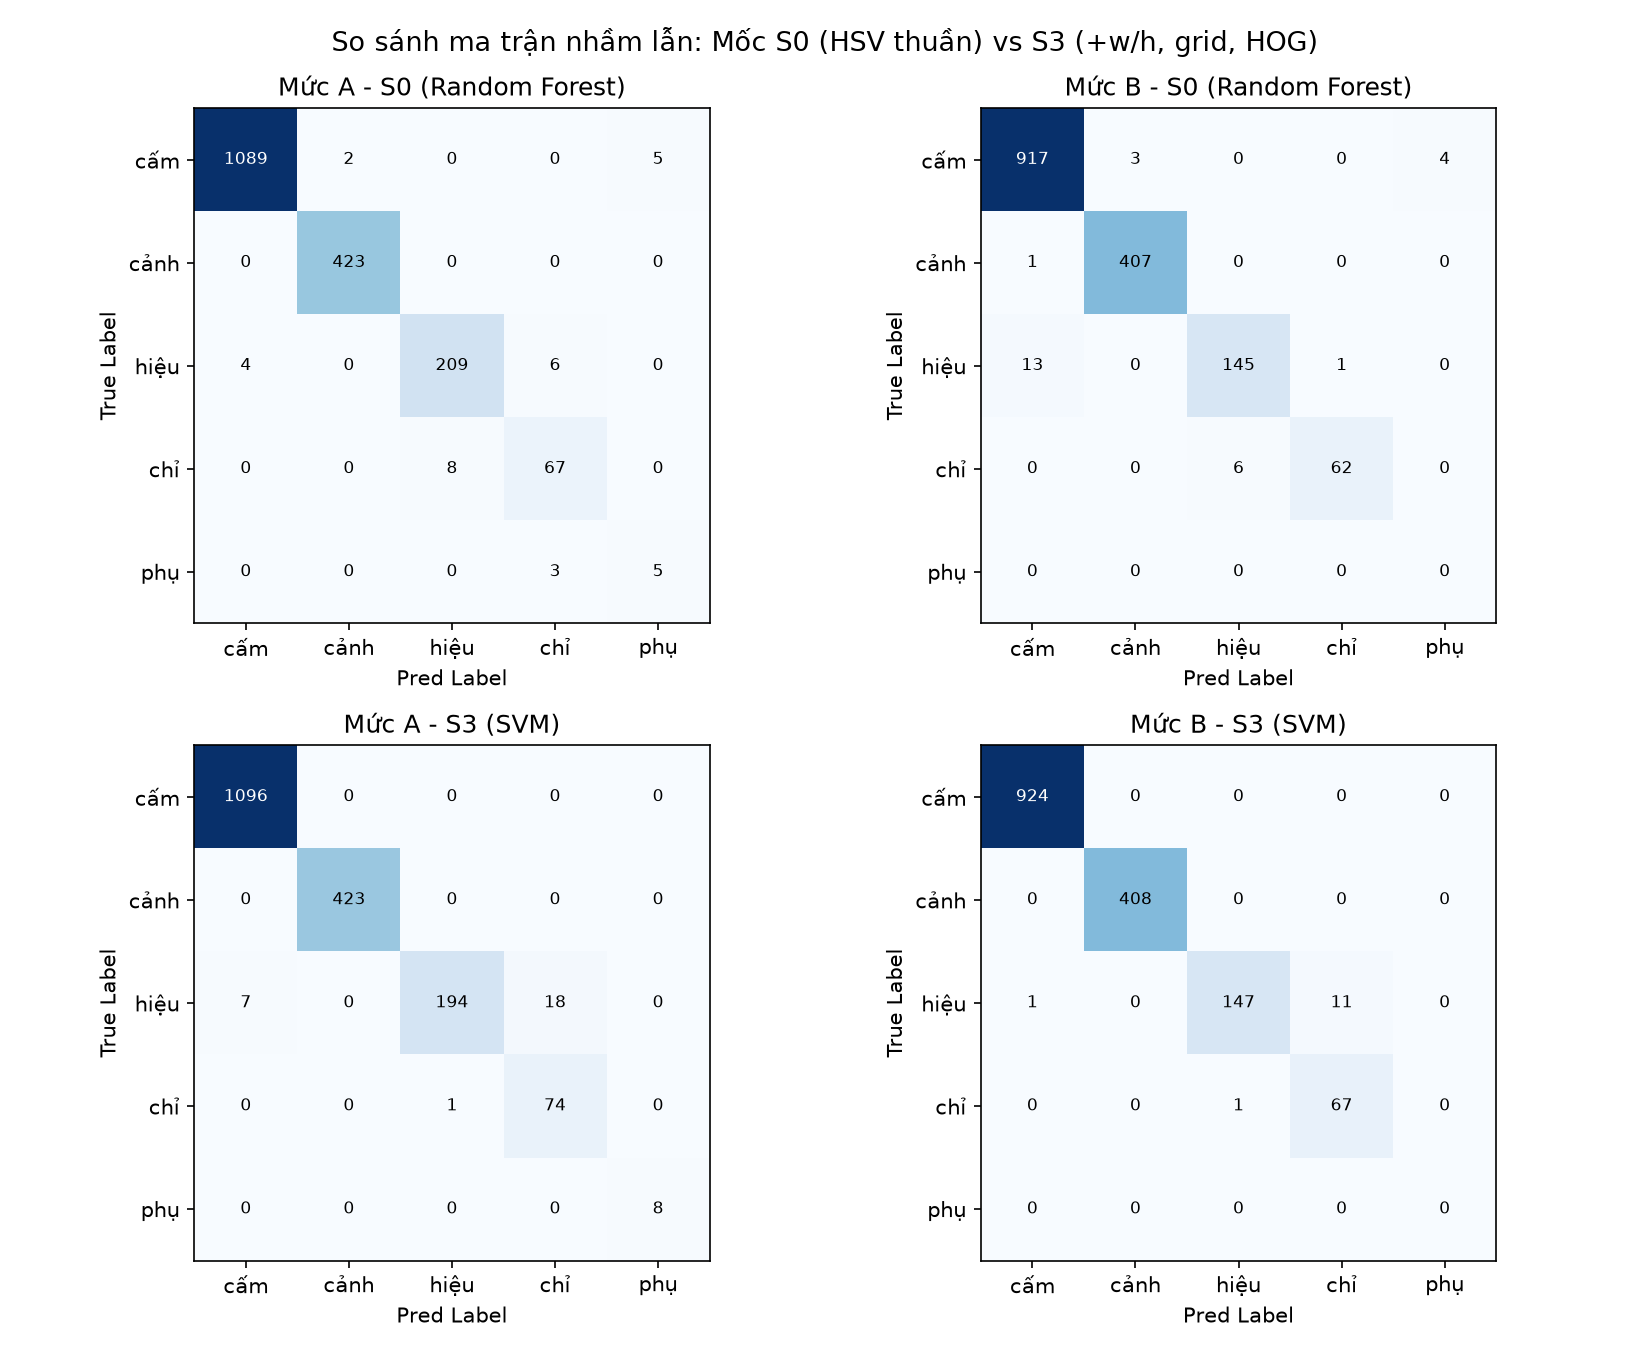
\includegraphics[width=0.92\textwidth]{graphics/sec4/f1_17_confusion_matrices_levels.png}
\caption{Ma trận nhầm lẫn chuẩn hóa của bộ phân loại SVM tại nấc $S3$: Mức A (ảnh ground-truth, trái) và Mức B (ảnh crop thực tế từ YOLO11s, phải).}
\label{fig:confusion_matrices_levels}
\end{figure}

\textbf{Đọc Hình~\ref{fig:confusion_matrices_levels}:}
Phân tích ma trận nhầm lẫn hé lộ sự bất đối xứng kỹ thuật quan trọng giữa hai chiều phân loại:
\begin{itemize}
    \item \textbf{Chiều Chỉ dẫn $\rightarrow$ Hiệu lệnh (Xanh chữ nhật/vuông bị đoán thành xanh tròn):} Đã được giải quyết gần như triệt để! Số ca nhầm giảm từ 20 ca ở $S0$ xuống chỉ còn \textbf{đúng 1 ca duy nhất ở $S3$} (đó là mẫu stem 0326, một biển chỉ dẫn quay đầu hình vuông bị chụp nghiêng góc khiến viền bị méo cong).
    \item \textbf{Chiều Hiệu lệnh $\rightarrow$ Chỉ dẫn (Xanh tròn bị đoán thành xanh chữ nhật/vuông):} Vẫn tồn tại \textbf{18 ca nhầm ở Mức A}. Phân tích truy vết mã nguồn cho thấy 100\% các ca này rơi vào biển hiệu lệnh kích thước nhỏ ($< 25\text{ px}$) ở cự ly xa (chuỗi stem 0365--0377). Khi crop ảnh con nhỏ được phóng đại nội suy lên $64 \times 64$, hiện tượng răng cưa biên (aliasing) biến đường cong tròn thành các cạnh gãy góc vuông, khiến bộ trích xuất HOG tạo ra phân bố gradient tương tự như góc cạnh biển chữ nhật.
    \item Đáng chú ý, ở \textbf{Mức B (1.559 crop từ YOLO)}, số ca nhầm lẫn giữa cặp này bằng \textbf{0 ca} (do các biển nhỏ xíu này đã bị detector bỏ sót ở Tầng 1 hoặc do crop thực tế có dải biên khác biệt). Do đó, khẳng định "giải quyết triệt để" chỉ đúng hoàn toàn trên tập crop Mức B, nhưng vẫn còn tồn đọng 19 ca nhầm ở tập ground-truth Mức A.
\end{itemize}

\begin{figure}[H]
\centering
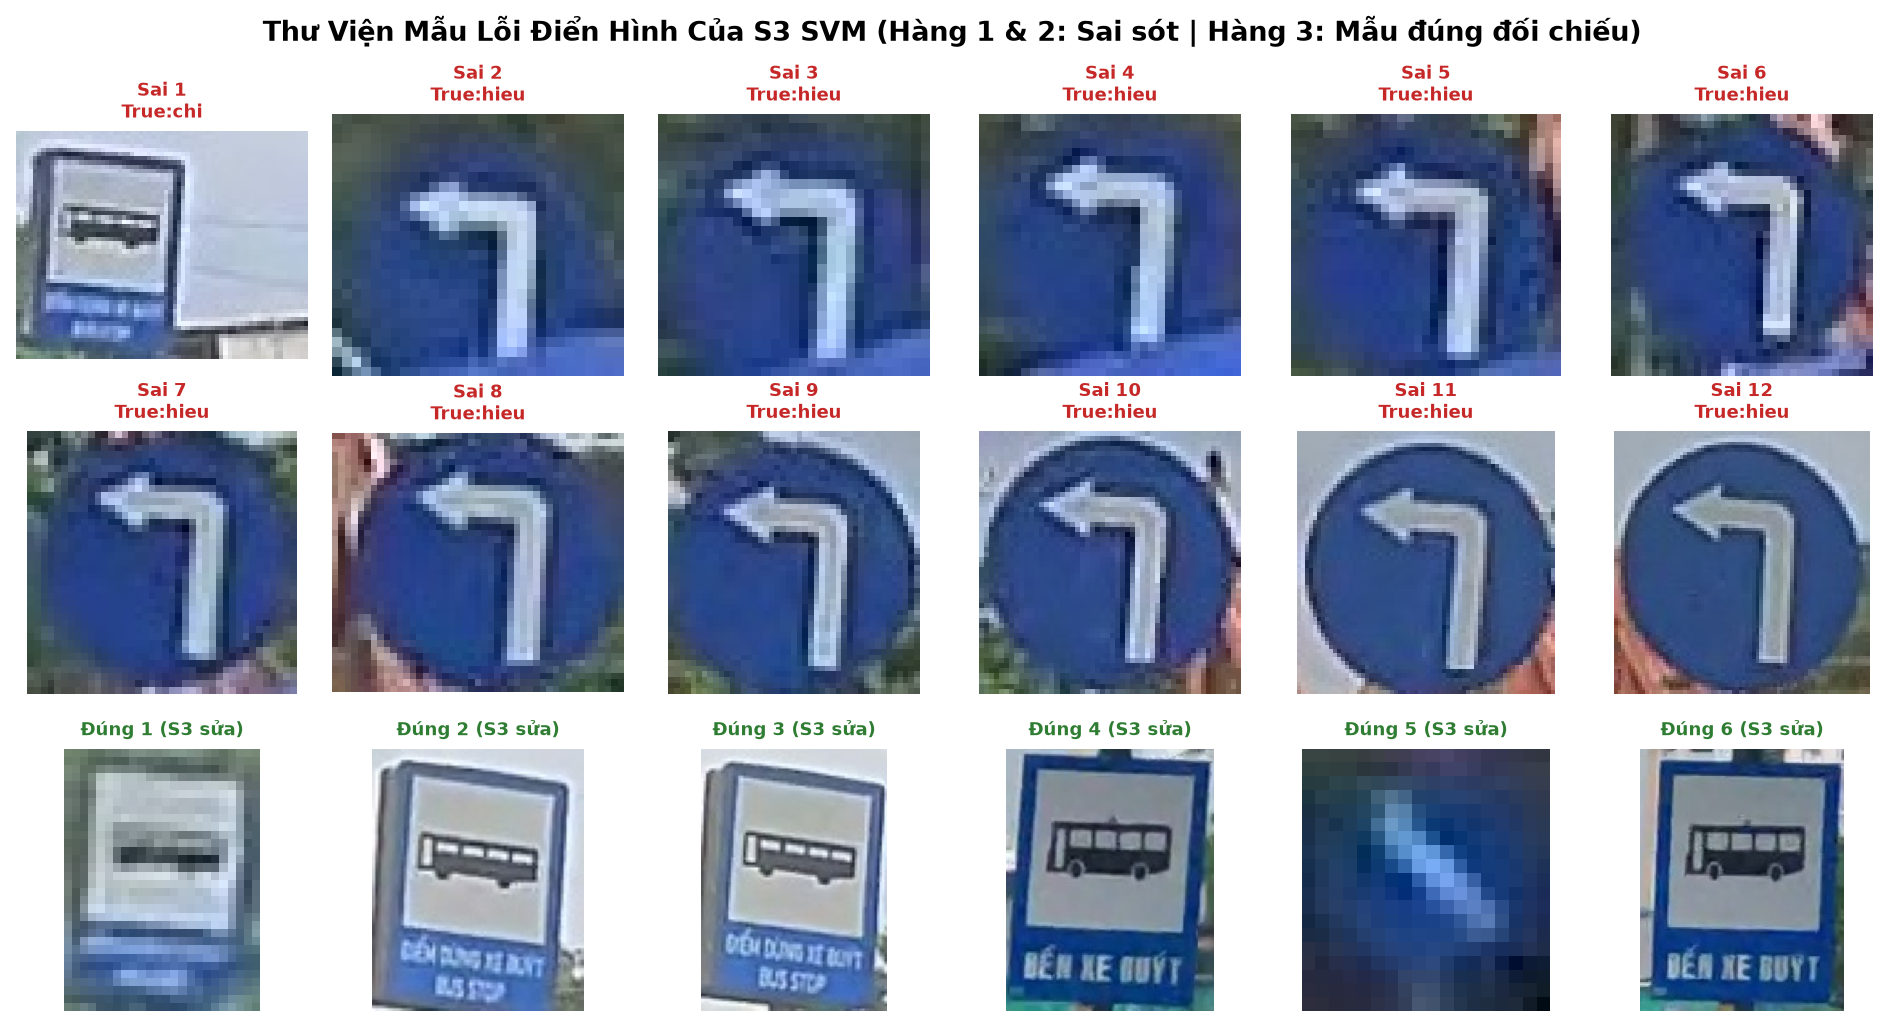
\includegraphics[width=0.92\textwidth]{graphics/sec4/f1_20_error_gallery_misclassified.png}
\caption{Thư viện trực quan các mẫu phân loại sai tiêu biểu của mô hình SVM $S3$ kèm mã định danh, nhãn gốc ground-truth và nhãn mô hình dự đoán.}
\label{fig:error_gallery}
\end{figure}

\textbf{Đọc Hình~\ref{fig:error_gallery}:}
Hình ảnh thực tế minh họa rõ nét các trường hợp lỗi: các biển hiệu lệnh tròn cự ly xa bị nhòe mờ dẫn tới đoán nhầm thành chỉ dẫn, biển cấm bị bóng cây che khuất làm biến đổi phân bố Hue, và một biển chỉ dẫn chụp ở góc nghiêng cực lớn bị nhận dạng nhầm thành hiệu lệnh.

% =========================================================================================
\subsection{Kết quả thực nghiệm Tầng 1: Đánh giá phân loại trên tập ROI độc lập (ROI Benchmark)}
\label{subsec:benchmark_roi}

Thực nghiệm đối chuẩn được thực hiện trên toàn bộ \textbf{1.813 mẫu ảnh ROI} thuộc tập Blind Test Block Split độc lập (không bị rò rỉ):

\begin{table}[H]
\centering
\small
\caption{Kết quả đối chuẩn phân loại trên tập Blind Test Block Split (1.813 mẫu ROI).}
\label{tab:roi_benchmark}
\begin{tabularx}{\textwidth}{|p{4.2cm}|>{\centering\arraybackslash}p{1.9cm}|>{\centering\arraybackslash}p{1.9cm}|>{\centering\arraybackslash}p{1.7cm}|>{\centering\arraybackslash}p{1.9cm}|>{\centering\arraybackslash}X|}
\hline
\textbf{Mô hình / Phương pháp} & \textbf{Accuracy} & \textbf{Precision} & \textbf{Recall} & \textbf{Macro-F1} & \textbf{Latency} \\
\hline
\textbf{Enhanced LeNet-5 (Học sâu)} & \textbf{98.73\%} & 94.46\% & \textbf{97.43\%} & \textbf{95.66\%} & \textbf{1.10 ms} \\
\hline
\textbf{Color + HOG + SVM (Truyền thống)} & 98.57\% & \textbf{94.82\%} & 96.81\% & 95.51\% & 2.63 ms \\
\hline
\end{tabularx}
\end{table}

\textbf{Phân tích kết quả chuyên sâu:}
\begin{itemize}
    \item \textbf{Enhanced LeNet-5:} Đạt hiệu năng dẫn đầu với độ chính xác tổng thể \textbf{98.73\%} và \textbf{95.66\%} Macro-F1. Tốc độ suy luận đạt mức ấn tượng \textbf{1.10 ms/mẫu} (tương đương \textbf{911.1 FPS}) trên CPU, chứng minh khả năng tối ưu hóa tính toán vượt bậc của kiến trúc CNN tùy biến.
    \item \textbf{Color + HOG + SVM:} Đạt độ chính xác rất cao \textbf{98.57\%} và \textbf{95.51\%} Macro-F1, tốc độ đạt \textbf{379.7 FPS}. Kết quả này chứng minh rằng khi kết hợp đúng đắn vector HOG định hướng với phân bố màu sắc cục bộ, phương pháp truyền thống hoàn toàn có thể cạnh tranh sòng phẳng với học sâu về độ chính xác nhận dạng trên ảnh con.
\end{itemize}

\begin{figure}[H]
\centering
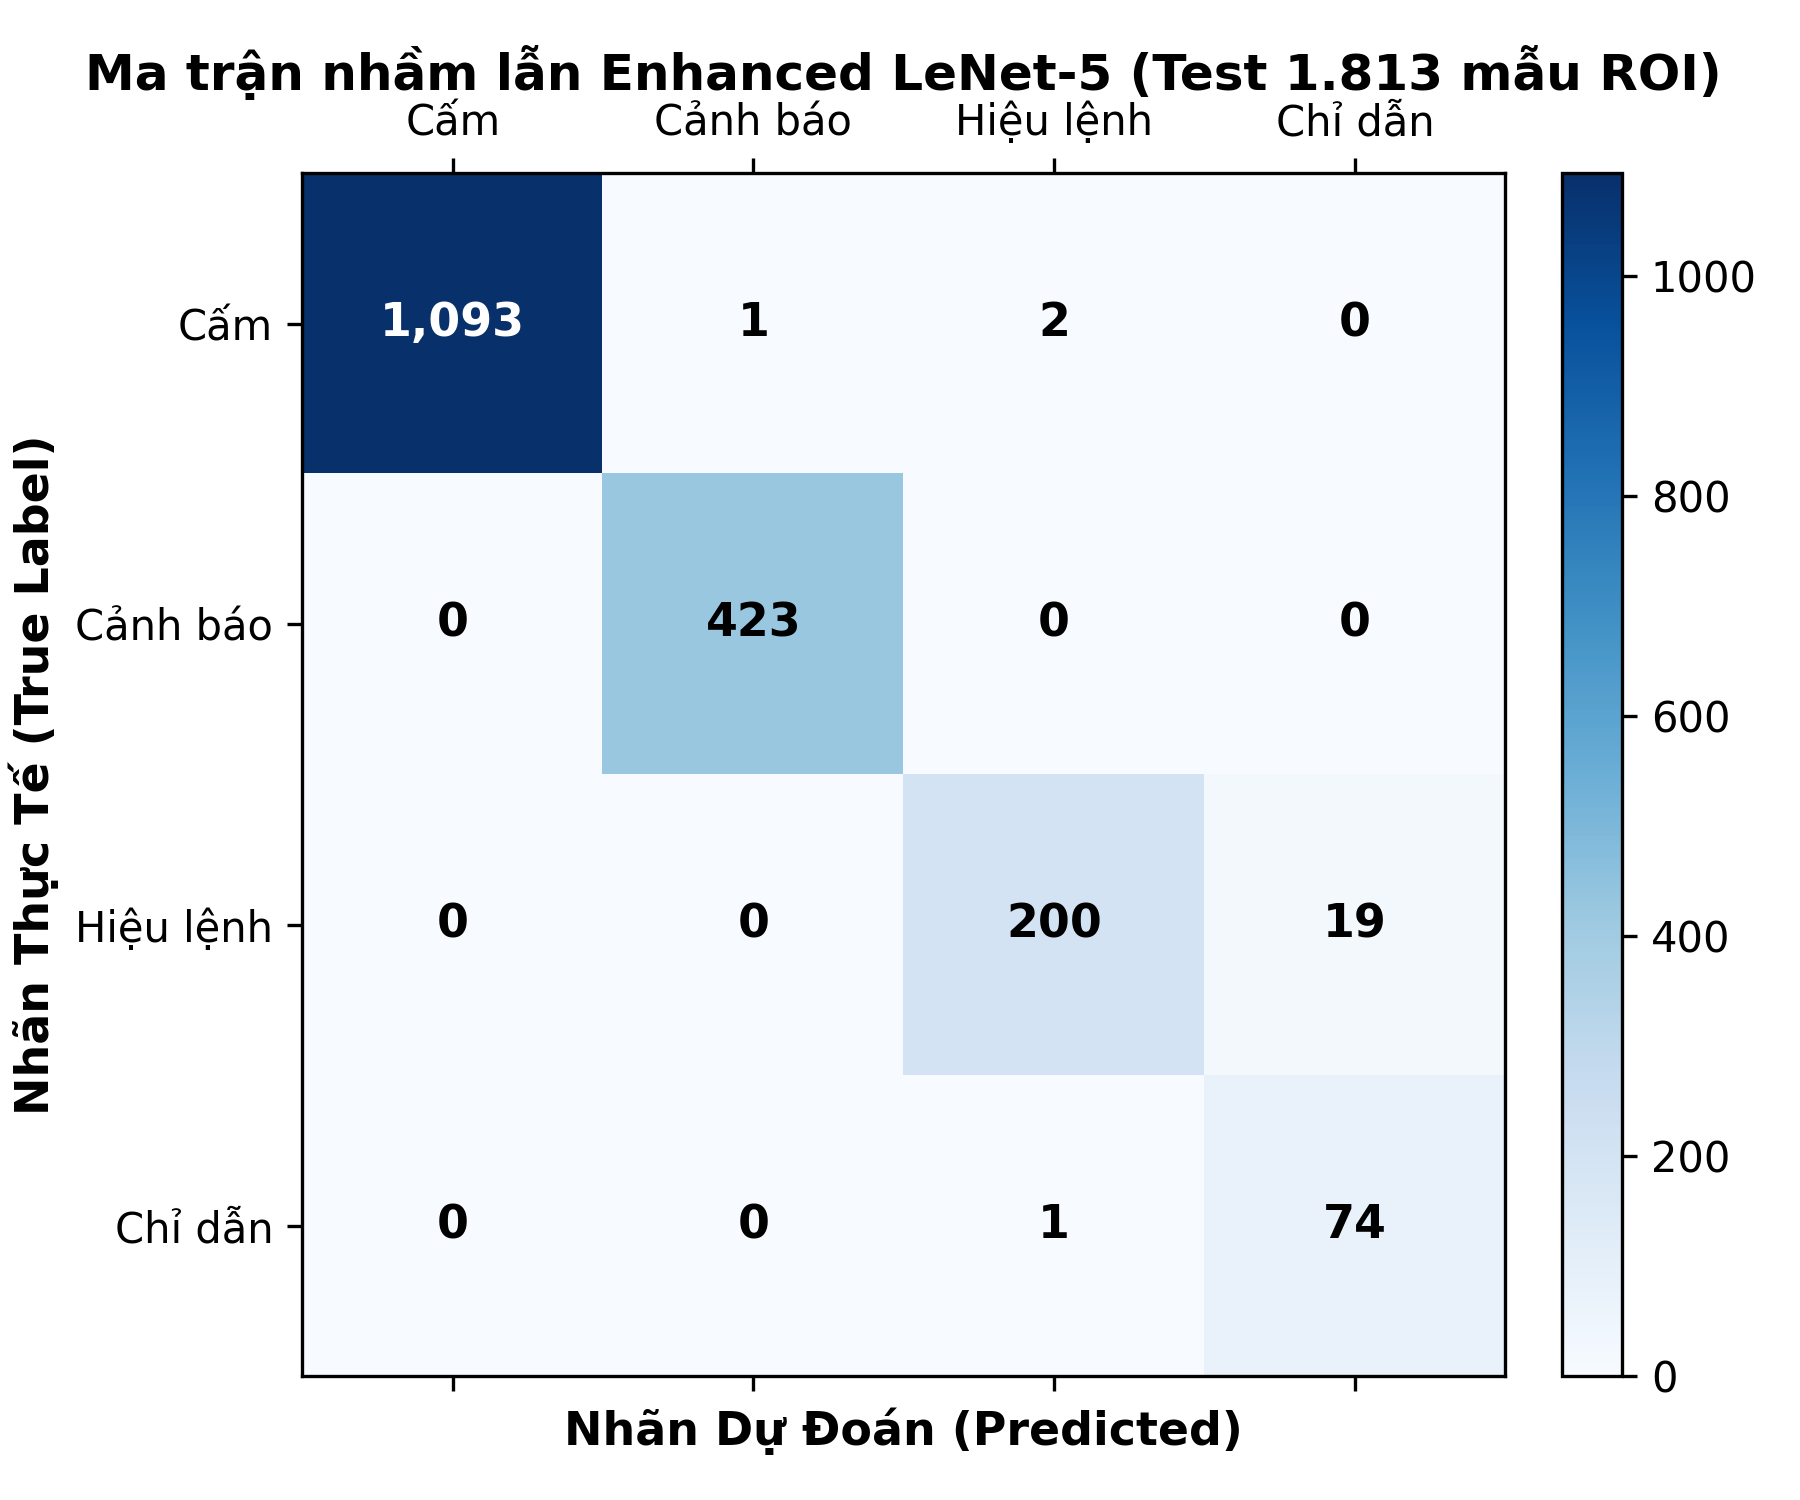
\includegraphics[width=0.58\textwidth]{graphics/sec4/f3_03_lenet_confusion_matrix.png}
\caption{Ma trận nhầm lẫn của mô hình Enhanced LeNet-5 trên tập Blind Test Block Split (1.813 mẫu ROI).}
\label{fig:lenet_confusion_matrix}
\end{figure}

\textbf{Đọc Hình~\ref{fig:lenet_confusion_matrix}:}
Ma trận nhầm lẫn của Enhanced LeNet-5 trên 1.813 mẫu test độc lập khẳng định sự vượt trội: nhóm Biển Cảnh Báo đạt độ chính xác tuyệt đối \textbf{100.0\%} (423/423 mẫu), Biển Cấm đạt \textbf{99.73\%} (1.093/1.096 mẫu). Đối với bài toán khó phân biệt giữa Biển Hiệu Lệnh và Biển Chỉ Dẫn (cùng màu xanh lam), mô hình phân loại đúng \textbf{200 / 219} mẫu Hiệu Lệnh và \textbf{74 / 75} mẫu Chỉ Dẫn, chỉ nhầm lẫn tổng cộng 20 mẫu cự ly xa bị nhòe mờ. Kết quả này bổ trợ hoàn hảo cho phân tích ma trận nhầm lẫn SVM tại Hình~\ref{fig:confusion_matrices_levels}.

\subsection{Kết quả thực nghiệm Tầng 2: Đánh giá toàn trình trên ảnh hiện trường (End-to-End Scene Benchmark)}
\label{subsec:benchmark_scene}

Thực nghiệm toàn trình được tiến hành trên \textbf{550 ảnh đường phố toàn cảnh} thuộc tập Blind Test, mô phỏng đúng luồng vận hành thực tế ngoài đường phố:

\begin{table}[H]
\centering
\small
\caption{Kết quả đối chuẩn toàn trình trên 550 ảnh đường phố toàn cảnh.}
\label{tab:scene_benchmark}
\begin{tabularx}{\textwidth}{|p{3.8cm}|p{2.2cm}|p{3.5cm}|>{\centering\arraybackslash}p{2.8cm}|>{\centering\arraybackslash}X|}
\hline
\textbf{Pipeline Toàn Trình} & \textbf{Bộ Định vị} & \textbf{Bộ Phân loại} & \textbf{Detection Recall} & \textbf{Acc $\mid$ Detection} \\
\hline
Two-Stage LeNet & YOLO11s & Enhanced LeNet-5 & 85.61\% & 99.40\% \\
\hline
Two-Stage SVM & YOLO11s & SVM (RBF) & 85.61\% & 99.17\% \\
\hline
\end{tabularx}
\end{table}

\textbf{Ý nghĩa của chỉ số đối chuẩn kép:} Việc đánh giá tách biệt hai tầng làm sáng tỏ một sự thật kỹ thuật quan trọng: Khi một biển báo đã được định vị thành công, cả hai bộ phân loại đều đạt độ chính xác gần như hoàn hảo ($\ge 99.17\%$). Điểm nghẽn hạn chế hiệu năng toàn hệ thống (End-to-End Recall $\approx 85\%$) nằm ở khâu định vị cự ly xa của YOLO11s chứ không phải do khâu phân loại.
